\documentclass[11.5pt]{sig-alternate} % sets document style to sig-alternate
% packages
% typesetting
%\usepackage{dirtytalk} % typset quotations easier (\say{stuff})
\usepackage{hanging} % hanging paragraphs
\usepackage[defaultlines=3,all]{nowidow} % avoid widows
\usepackage[pdfpagelabels=false]{hyperref} % produce hypertext links, includes backref and nameref
\usepackage{xurl} % defines url linebreaks, loads url package
\usepackage{microtype}
% layout
%\usepackage{enumitem} % control layout of itemize, enumerate, description
\usepackage{fancyhdr} % control page headers and footers
\usepackage{float} % improved interface for floating objects
%\usepackage{multicol} % intermix single and multiple column pages
% language
\usepackage[utf8]{inputenc} % accept different input encodings
\usepackage[english]{babel} % multilanguage support
% misc
\usepackage{graphicx} % builds upon graphics package, \includegraphics
%\usepackage{lastpage} % reference number of pages
%\usepackage{comment} % exclude portions of text (?)
\usepackage{xcolor} % color extensions
\usepackage[backend=biber, style=apa]{biblatex} % sophisticated bibliographies % necessary for HTML to display author info and date on abstract page
\usepackage{csquotes} % advanced quotations, makes biblatex happy
\usepackage{authblk} % support for footnote style author/affiliation
% tables and figures
\usepackage{tabularray}
\usepackage{array} % extend array and tabular environments
\usepackage{caption} % customize captions in figures and tables (rotating captions, sideways captions, etc)
%\usepackage{cuted} % allow mixing of \onecolumn and \twocolumn on same page
\usepackage{multirow} % create tabular cells spanning multiple rows
%\usepackage{subfigure} % deprecated, support for manipulation of small figures
%\usepackage{tabularx} % extension of tabular with column designator "x", creates paragraph-like column whose width automatically expands
%\usepackage{wrapfig} % allows figures or tables to have text wrapped around them
%\usepackage{booktabs} % better rules
% dummy text
%\usepackage{blindtext} % blind text dummy text
%\usepackage{kantlipsum} % Kant style dummy text
%\usepackage{lipsum} %lorem ipsum dummy text
% other helpful packages may be booktabs, longtable, longtabu, microtype

\pagestyle{fancy} % sets pagestyle to fancy for fancy headers and footers

% header and footer
% modern way to set header image
\renewcommand{\headrulewidth}{0pt} % defines thickness of line under header
\renewcommand{\footrulewidth}{0pt} % defines thickness of line above header
\setlength\headheight{80.0pt} % sets height between top margin and header image, effectively moves page contents down
\addtolength{\textheight}{-80.0pt} % seems to affect the lower height. maybe only works properly if footer numbers enabled?
\fancyhf{}
\fancyhead[CE, CO]{
\includegraphics[width=\textwidth]{headerImage.png}}
% footer
%\fancyfoot[LE,LO]{Article Title Here \\ DOI: }% left footer article title and doi
%\fancyfoot[CE,CO]{{}} % center footer empty
%\fancyfoot[RE,RO]{\thepage} % right footer page numbers
%\pagenumbering{arabic} % arabic (1, 2, 3) numbering in footer

\hypersetup{colorlinks=true,urlcolor=blue} % sets link color to blue
\urlstyle{same} % sets url typeface to same as rest of text

% set caption and figure to italics, label bold, left align captions, does not transfer to HTML
\DeclareCaptionFormat{custom}
{
    \textbf{\textit{\large #1#2}}\textit{\large #3} % #1 is the "Table 1" or "Figure 1" part, #2 is the separator (":"), #3 is the caption
}
\captionsetup{format=custom}
\captionsetup{justification = raggedright, singlelinecheck = false}
 
\let\oldabstract\abstract
\let\oldendabstract\endabstract
\makeatletter
\renewenvironment{abstract}
{\renewenvironment{quotation}%
               {\list{}{\addtolength{\leftmargin}{1em} % change this value to add or remove length to the the default
                        \listparindent 1.5em%
                        \itemindent    \listparindent%
                        \rightmargin   \leftmargin%
                        \parsep        \z@ \@plus\p@}%
                \item\relax}%
               {\endlist}%
\oldabstract}
{\oldendabstract}
\makeatother


\begin{document}

\title{Use of Scientific Argumentation by Deaf/Hard-of-Hearing Students in Environmental Science Topics}

\author[1]{\large \color{blue}Annemarie D. Ross}
\author[1]{\large \color{blue}Todd Pagano}
\author[2]{\large \color{blue}Randy Yerrick}

\affil[1]{National Technical Institute for the Deaf Rochester Institute of Technology}
\affil[2]{Department of Learning and Instruction University at Buffalo}
\toappear{}
%% ABSTRACT
\maketitle
\begin{@twocolumnfalse} 
\begin{abstract}
\item 
\textit {Deaf/hard-of-hearing postsecondary students may have some misconceptions surrounding scientific concepts that might be partially ascribed to a lack of access to culturally-responsive forms of pedagogy. The Deaf and hard-of-hearing community is diverse in communication modes, including those who use American Sign Language as their primary language, and therefore, some students from this population may display characteristics similar to English Language Learners. Through classroom discourse analyses and interviews, we found a general lack of persuasion characteristics used by most students in an environmental science unit, and that the lack of higher-level scientific argumentation skills seemed to be related to students not having prior exposure to persuasive strategies. With the goal of improving Deaf and hard-of-hearing students’ equitable access to quality science education, strategies should be considered in teaching approaches, and results suggest the need to include scientific argumentation tasks within sociocultural learning contexts. Ultimately, the goal is to work toward educating and engaging Deaf and hard-of-hearing students in science inquiry and improving the environmental scientific literacy of this underrepresented group.}
\\ \\
Keywords: environmental science education; Deaf and hard-of-hearing education; English Language Learners; argumentation; persuasion; culturally-responsive teaching
\end{abstract}
\end{@twocolumnfalse}

%% AUTHOR INFORMATION

\textbf{*Corresponding Author, Annemarie D. Ross} \\
\href{mailto: adrnts@rit.edu }{(adrnts@rit.edu)} \\
\textit{Submitted  October 18, 2019} \\
\textit{Accepted November 18, 2019} \\
\textit{Published online February 24, 2020} \\
\textit{DOI:10.14448/jsesd.12.0005} \\
\pagebreak
\clearpage

\begin{large}
\section*{INTRODUCTION}
    
As a member of the Deaf and Hard-of-Hearing community, I (the first author) take my role seriously as an advocate for a minority group by incorporating quality teaching practices in science to benefit Deaf and Hard-of-Hearing students. I teach this group of students in the Laboratory Science Technology (LST) program at the National Technical Institute for the Deaf (NTID) at the Rochester Institute of Technology (RIT); established to provide Associate’s degrees for Deaf and hard-of-hearing students and/or to provide preparation for their continued baccalaureate studies (Pagano, 2017; Pagano, Ross, \& O’Neill, 2012). With over 1,100 Deaf and hard-of-hearing students enrolled on campus (NTID, 2018), our institution provides a unique context for studies in Deaf and hard-of-hearing pedagogy. This, in turn, provides an ideal place for my research and teaching to inform one another in my quest to provide equitable access to quality science education for my students. 

As a science professor, I began to consider the application of discourse and literacy research to the cause of forwarding progressive pedagogies in my classroom. Within such a wide array of possible scientific disciplines, sustainability and developing environmentally-literate community members are current trends in higher education (Buckley, 2019; Kanwar \& Asad, 2019; Lozano, Barreiro-Gen, Lozano, \& Sammalisto, 2019; Tejedor et al., 2019). Knowledge and understanding of climate science topics and other sustainability-related topics are vital to developing more “green thinking” community participants. Prior to the specific pedagogical strategies employed in this project, we conducted a preliminary survey that tested certain topical environmental science/sustainability-related knowledge. Results showed a difference in understanding/knowledge between groups of hearing and Deaf/hard-of-hearing students on RIT campus (A. D. Ross, Yerrick, \& Pagano, 2019). We subsequently incorporated some environmental science classroom activities and examined the application of historical and emerging frameworks for understanding the students’ responses to shifts in my pedagogy. This work included a multi-year case study conducted in my classroom based upon the following assumptions: 1)Deaf and hard-of-hearing students often receive basic traditional science instruction and are not as often exposed to progressive, sociocultural (Vygotskiĭ, 1987), nor culturally-responsive forms of pedagogy. 2)Science is a specialized discourse. University science classrooms are rife with well-established norms which often constrain access to underrepresented students of science. 3)Learning and acquiring new discourse norms of thinking, speaking, and acting are cultural acts and require specific lenses through which to view starts, stops, and progress along the way.

One of the constraints faced by the Deaf and hard-of-hearing community is the documented writing challenges for some members when using the English language (Marschark, Tang, \& Knoors, 2014). While such a lag between the written and expressive language is common during the process of learning a new language, it is also a challenge which emerges because the students are often dependent on American Sign Language (ASL), which does not have a written form (Plaza-Pust, 2014; Stokoe, 1978), setting it apart from most other languages. Deaf and hard-of-hearing students’ challenges can be comparable to those experienced by English Language Learners (ELL), in that many Deaf and hard-of-hearing students use ASL as their primary language and English as their secondary language. Quinn et.al. (2012) provide a list of features to include for science language learning for ELL students, which can be similar for general English language learning for Deaf and hard-of-hearing students (Knoors, 2013); such as the emphasis on science vocabulary, multiple modes of representation (like visual representations), use of literary strategies, as well as home language and culture connections within the science classroom. We therefore believe that it is a reasonable conjecture that ELL strategies may be useful in exploring ways to improve environmental science educational access for Deaf and hard-of-hearing students. 

With the intent to find ways to remedy gaps in the science education of this minority population with social and culturally-responsive pedagogies, our guiding question for our project became: How do Deaf and hard-of-hearing students respond to the environmental science-focused, ELL teaching approach, when engaged with an online climate science resource, and more specifically, what scientific argumentation strategies were observed in students’ discourse during the climate science assignment? To answer our study question, we implemented classroom strategies into the curriculum to help students learn climate science concepts, collected data on student responses to the strategies, and uncovered that the students possessed varying levels of persuasion skills. It is interesting to note that scientific concepts surrounding climate change are excellent venues for the evaluation of scientific argumentation and persuasion skills in students because they are highly relatable to what is seen in the “real-world”, and the related science is often seen under scrutiny by the public in different media circles. 

\section*{BACKGROUND}

A significant percentage of the United States’ population has some form of hearing loss, with 960,649 individuals in the age range of secondary and post-secondary students (5-34 years old) (U.S.Census Bureau, 2013). The English (reading and writing) and mathematical testing statistics among Deaf and hard-of-hearing students demonstrate the need for improving science educational access (SRI International, 2006a; SRI, International, 2006b). These gaps and general public perception can be part of the reason that the Deaf and hard-of-hearing community is still viewed by the majority population as a ‘disabilities community’. However, we do not agree with this notion and, like others (Abes \& Wallace, 2018; Abrokwa, 2018; Kerschbaum \& Price, 2017; Munro, Knox, \& Lowe, 2008; Nuwagaba \& Rule, 2016), instead adopt Oliver’s (1986) Social Theory of Disability which argues that disability is a function of society’s lack of inclusion during the design process; such as in policies, buildings, and the like. We agree with Oliver (1986) that educators should intentionally depart from viewing deafness as a disability to that of a minority group with their own culture, language and identity. Deaf and hard-of-hearing students are, under such a culturally-responsive teaching framework, one of many marginalized groups of students in need of supporting strategies that level the educational playing field to that of their hearing peers. Note that we are aware of the common preference to use “people first” language and support the rationale, however, since the Deaf community takes pride in the Deaf label as a part of a cultural community, in this paper, we use “identity-first” approach in that we use Deaf as the initial identifier (as in “Deaf and hard-of-hearing students”, for example). Also note that we use the capital letter, D, in a sociocultural context to signify those who associate with the Deaf culture, while the term, hard-of-hearing, represents those who might be deaf or hard-of-hearing, but do not entirely associate with the Deaf culture. Additionally, because our study design was not to isolate student performance based on their Deaf, deaf, or hard-of-hearing identity, the term “deaf and hard-of-hearing” is used here to include students who may or may not associate with Deaf culture and/or are hard-of-hearing.

There is a history of marginalization by stigma perhaps due to the categorization of ASL, denying it as a \textit{language} until the late 1970s when Stokoe published the first linguistic analysis (Stokoe, 1978). ASL was seen as signs following the syntax of English, thus not as a language of its own, or as a form of “gesture”, which Stokoe (1978) refuted with his documentation of the unique syntax and linguistic features of ASL. Yet, as we make any suggestions that ASL users may benefit from pedagogical research done on the ELL community, we must understand how the application of ELL strategies may affect the ASL-primary learners, i.e. keeping in mind that ASL is neither an audibly-based language nor does it have a written component (as are cases in most other languages of the ELL community). 

While there may be many explanations for the comparative differences with student national achievement testing results, we believe that some of the achievement gaps related to Deaf and hard-of-hearing students might be better explained from the Critical Response Theory (CRT) perspective— as a lack of opportunity rather than a deficit comparison. Therefore, current Deaf and hard-of-hearing science pedagogical research offers opportunities to impact our notions of socially responsible, equitable education and to bring necessary evidence-based tools to the classroom.

\subsection*{Science Education Standards, Scientific Argumentation, and English Language Learners}

Contemporary reforms, such as the Next Generation Science Standards and the Common Core State Standards (National Governors Association Center for Best Practices \& Council of Chief State School Officers, 2010; NGSS Lead States, 2013) in the U.S. call for a reworking of science classroom discourse. The standard raised for educating the next generation of scientists is rooted in the active participation of students in applying scientific and mathematical constructs to contemporary issues. According to reform visions, the classroom is to be a place where students practice the application of evidence and critical analysis to the solution of real-world problems. Such a vision involves student thinking and classroom discourse through which scientific argumentation can be a lens to observe students’ critical thinking and scientific literacy in practice. Acts of scientific argumentation involve the process of discussing how, and if, evidence supports a scientific hypothesis or warrant. . The mechanism of argumentation involves critique and reflection— affording participants the opportunity to engage in the exploration of both the epistemological and ontological processes of constructing knowledge (Cavagnetto \& Kurtz, 2016; Katherine L. McNeill \& Krajcik, 2009; Sampson \& Walker, 2012). It is no longer deemed sound practice to view science teaching as the transmission of facts, accumulation and mastery of scientific specialized vocabulary, nor expert practicing of process skills (K.L McNeill, Gonzalez, Katsh-Singer, \& Loper, n.d.). Rather, science classroom discourse should be “a way of talking about a subject using a particular thematic pattern” (Lemke, 1990, p. 125; K.L McNeill, Lizotte, Krajcik, \& Marx, 2006). As an individual develops expertise in a field, there is a thematic pattern for which they need to be familiar in order to communicate with others in the field (Grooms, Sampson, \& Enderle, 2018). Novice scientists need to learn how to communicate and write within this argumentation genre, using appropriate terms or phrases within the context and constructs where they are appropriately applied (K.L McNeill et al., n.d.). Some examples include “I hypothesize,” “this figure shows,” or “the evidence refutes.”

It can be a challenge to make large argumentation shifts in the scientific articulation of any student (Duschl \& Osborne, 2002; Quinn et al., 2012; Tolbert, Stoddart, Lyon, \& Solis, 2014), as the use of persuasion within science discourse is a form of learning at a higher cognitive level compared to the descriptive or stating of facts. It may even be more difficult for some Deaf and hard-of-hearing students as ELL. That is, some Deaf and hard-of-hearing learners not only need to tackle the scientific discourse that is required for a successful career, they often also have to address writing in English from a second-language perspective. In these cases, ASL may be their first language (L1) with English as their second language (L2), requiring associations beyond vocabulary to master English in the written form as well as the usage of scientific discourse. Linguistically, that is quite a feat. Projects to address such linguistic barriers have been conducted in the field, and while not part of the currently discussed study, as it relates to environmental science, a team at RIT/NTID has worked to develop a collection of sustainability-related technical terms in ASL (“RIT/NTID ASL CORE,” n.d.) through a National Science Foundation supported Innovations at the Nexus of Food, Energy and Water Systems (INFEWS) grant (\textit{INFEWS CBET-1639391}).

There are limited studies aimed at establishing whether or not the strategies for the hearing ELL community (also referred to as unimodal bilinguals – proficiency in two spoken languages), will work for the Deaf and hard-of-hearing community (bimodal bilinguals – proficiency in one spoken and one visual language). The neurological processing of ASL occurs in the same regions of the brain as that of spoken language processing (Emmorey, 2002), which may cause one to assume that what works with the hearing community for language transfer would work with the Deaf and hard-of-hearing community. However, research also shows that the translation from using ASL to writing in English is not as effective as when individuals use their respective languages in the hearing ELL community (Singleton, Morgan, DeGello, Wiles, \& Rivers, 2004), with speculation of the cause to be “…modality differences lead to differences, for example, in the degree of sequential versus simultaneous ordering of lexical elements” (Marschark et al., 2014, p. 4). Lexical elements refer to the order of the sentence/word structure, which is different when comparing ASL and English structure. 

Treating English, and specifically that within the sciences, as a second language for Deaf and hard-of-hearing students may offer some inroads that past educational trajectories have failed to produce. Learning English, or learning scientific argumentation in English (rather than ASL), does not mean learning to \textit{speak} English. So, unlike most in the ELL community, primary-ASL users have the unique challenge of navigating from a visual language, with no written component, to writing in English. As the literature suggests, speaking a language helps to write in a language, but ASL users do not have that transfer support (Marschark et al., 2014; Mayer \& Akamatsu, 1999). Our study does not represent a linguistic analysis from the perspective of a specialist in the field. Rather, it is an applied approach to leverage new pedagogical techniques to promote new notions of scientific discourse for Deaf and hard-of-hearing students. 

There is research to support our conjecture relating Deaf and hard-of-hearing to ELL learners, as the research refers to Deaf and hard-of-hearing ELL as bilingual learners (Marschark et al., 2014), including studies which discuss strategies to use for Deaf and hard-of-hearing ELL (Cannon \& Guardino, 2012), as well as consideration of sign languages as a modality of input for L1 or L2 acquisition (Barcroft \& Wong, 2013). We also engage students in writing, as an opportunity to write using scientific terms like a scientist; which represents a higher level of applying both science discourse and the use of the English language. Hence, mastering scientific discourse through a form of writing-to-learn-science process (Connolly \& Vilardi, 1989) may be paramount in working toward leveling the playing field for Deaf and hard-of-hearing student access to science participation, professional preparation and advancement in careers. 

\section*{METHODS}

This qualitative study received Internal Review Board (IRB) approval and began as an environmental science activity in which we explored the use of the American Chemical Society’s (ACS) Climate Science Toolkit web resource (“ACS Climate Science Toolkit—American Chemical Society,” 2008) to supplement traditional pedagogical materials in the teaching of climate science topics at NTID. The ACS designed the Climate Science Toolkit for the general public to better understand evidence supporting the impact of human activity on the climate (“ACS Climate Science Toolkit—American Chemical Society,” 2008). 

\subsection*{Implementation of ELL and Sociocultural Strategies}

This project involved two phases of curriculum design, each involving activity implementation, data collection/analysis, and reflection. We refer to the students who participated in the different phases as being in Cohort One and Two, respectively. The activity timeline for both cohorts were the same; one class period to explore the ACS Toolkit website, with a second to work on their written wiki platform, and, a third class period to present their wiki projects through a presentation in their primary or preferred language (ASL or English). A wiki is an online Blackboard platform that allows students to directly link to sources as they write; giving a different medium for writing which allows more flexibility to incorporate website visuals/videos.  The first part of the activity incorporated the ACS Climate Science Toolkit website and the school’s wiki platform from which information related to student writing was collected and analyzed. For Cohort One data collection was comprised of examining the students’ use of the ACS Toolkit website within student teams, who also presented together. 

Based on our observations of the first cohort and with consultation of the literature, we were led to the framework, Scaffolded Knowledge Integration (SKI) (Bell \& Linn, 2000; Linn, 1995). Such an approach treats knowledge as co-constructed between instructor and students and emphasizes the use of directed prompts to encourage higher level thinking and the use of evidence within an argumentation context. Bell and Linn (2000) promote four specific elements during the implementation of SKI to facilitate argumentation in ways similar to current science education reform standards. These four elements include: 1)providing connections to students’ personal experiences, 2)making thinking visible, 3)promoting autonomy, and 4)promoting effective social interactions for learning. We adapted our study design and attended to these elements in our work in the following ways for the second cohort of students: 1)Students were provided with writing prompts that relate to their experiences as Deaf and hard-of-hearing citizens, as well as exposure to significant figures (e.g. referencing comments from the Pope). 2)Students were assigned the use of the wiki tool for implementation of visual media, including pictures, figures, charts, videos, and other modes of visible data forms from the ACS Toolkit. 3)Students individually (not in teams for the second cohort) presented their data from the wiki to the classroom peers and instructor in order to support their position on climate science topics. 

With some overlap of the SKI design, we also engaged our Deaf and hard-of-hearing students with integrated writing practices using ELL strategies as recommended in the literature using five components (Quinn et al., 2012): 1)Literacy strategies that incorporate both science and literacy learning, while understanding that “literacy” covers talking as well as thinking, in this case, literacy strategies are incorporated through the use of reading the toolkit and writing on the wiki. 2)Language support through providing multiple language venues to communicate science through examples like the visual graphs/pictures from the toolkit, the text from each other’s wiki’s; all while using environmental science specific discourse. 3)Strategies which incorporate science-specific discourse, in this case, environmental science, through both a writing and presentation venue. 4)Support of students’ native language through the option to use ASL as students presented to each other. 5)Connections to students’ familiar culture through the added writing prompts.

Additional changes in the second phase were individual, instead of team, wiki/presentations for more tailored data to understand individual student performance, as they were explicitly told to persuade their audience on concepts related to climate science (while not explicitly taught how to persuade). 

\subsection*{Sample}

Participants in the two cohorts were a total of 27 first- or second-year students enrolled in the LST program at NTID. Class sizes are purposely kept small as part of NTID’s mission and Cohort One had 14 students, while Cohort Two had 13 students. There is value in studies of this size (including case studies) since we are dealing with a low-incidence population (Deaf and hard-of-hearing postsecondary students (Snyder, de Brey, \& Dillow, 2016)) in which it is difficult to achieve a study with larger sample sizes. The Deaf and hard-of-hearing students in this study have a wide variety of communication backgrounds and preferences. As discussed as a limitation, and due in part to sample size in this case study, we did not separate the communication styles of the students beyond noting that they are all “Deaf and hard-of-hearings” students. Further, these students have varied science knowledge that stems from diverse high school backgrounds. We employed the assistance of interviewers and co-instructors to manage and standardize data collection and instruction. We conducted follow-up interviews to ground our interpretations (Mishler, 1986), so as to avoid incorrectly inferring alternate interpretations from their intended meaning and to assure that our understanding closely aligned to participants’ own interpretation. Students were chosen for these interviews based on their availability as well as trying to get a range of differences in terms of their language preferences (ASL/English). To get a better understanding of their high school backgrounds, we followed-up with debriefing interviews and member-checking to understand how, why, and when students chose to use persuasive statements and data in their classroom tasks. 

\subsection*{Data Analysis}

For both cohorts, we conducted interviews using Spradley’s coding methodology (Spradley, 1980) and we incorporated Berland and Reiser’s (2009) persuasive statement coding. Interestingly, the findings for the Deaf and hard-of-hearing students in our study had some similarities to those non-Deaf and hard-of-hearing students reported by the authors (Berland \& Reiser, 2009), in that students did not always move to a level of persuasion, which led to the incorporation of direct argumentation strategies for the second cohort. In order to interpret the students’ classroom writing, participation, and general acquisition of sustainability-related argumentation skills, we coded classroom interactions, interview data, and student-generated learning artifacts using Spradley’s (1980) process of domain analysis (shown in the Appendix). The data collection did vary some between cohorts in that the first cohort only had written artifacts from the wiki, with debriefing interviews. In addition to those data sources, the second cohort had classroom videorecordings of the teacher, students and presentations analyzed using Erickson’s videorecording methodology (Erickson, 2012). Throughout the iterative process of refining the planning of the teaching activities for two cohorts of students, studying the effects, and incorporating reflective pedagogy; we were led to a better understanding of the nature of the differences in the students related to how they approached the instructional tasks and how they interpreted the resources that were provided for them. 

As the authors ascertained the ‘explainer’ and ‘persuader’ tendencies (defined later), those tendencies informed improvements to the design of the curriculum for the second cohort– where students were asked to ‘persuade’ in their assignments and additional data was collected in the form of classroom video recordings. The performance of example students (whose names have been changed to protect their identity) from this second cohort are displayed below in figures as scientific argumentation vectors. These are radar plots that demonstrate their responses (i.e., counts of each type of response on each axis) to different assignments in the climate science project. The vector plots help to visualize and discuss students’ performance (in magnitude/count) and generally in tendency (direction) as ‘persuaders’. Incidences of the use of persuasive language in the students’ assignments were determined and quantified by the authors.

\section*{RESULTS AND DISCUSSION}

Within the activities in this activity, students were provided an environmental science project that incorporated ELL strategies from a sociocultural perspective (the SKI framework). Students were provided a wiki platform to share evidence of climate change through the use of visual media. Such visual media gave these students another form of language support (both SKI and ELL elements) to convey their thoughts. The added writing prompts provided personal experiences for them to connect to (also SKI and ELL elements) as community participants. Overall, attention to the SKI and ELL strategies, which already incorporated the reform standards, provided us with the ability to tailor our curriculum so that students benefitted from an enhanced learning experience.

\subsection*{Students’ Scientific Argumentation Characteristics}

As we took to understand the perspective of students throughout their learning experience with the activities, we were led to examine how they had approached their climate science project. Throughout the interviews of students in Cohort One, two differentiating groups of students became apparent surrounding their approaches to the assigned tasks, and subsequently, questions arose related to their use of scientific argumentation. While at first, we recognized the efforts that needed to be taken to be more explicit in the writing assignments for the second cohort of students (i.e. to prompt students to use argumentation using home cultural references as recommended by ELL literature), we came to eventually understand that some students generally struggle (or don’t choose) to use scientific argumentation conventions (e.g., evidence, persuasion) in their discussion of scientific concepts. We explored the differences in our students’ approach to the assignments—differences which may have profound impacts on the access some of our students have to enhanced educational opportunities.

From the students in the first cohort, we observed that student performance on the climate science activities started to show differentiation into two categories of responses. We observed the categorization of student response into language associated with ‘explainers’ (predominantly stating facts) and ‘persuaders’ (using persuasive statements to convince others of a concept/topic/theory). We will be using such labels to demonstrate the range of tools the students use between that of ‘explainers’ and ‘persuaders’. It is important to note that we are not implying that ‘explainers’ and ‘persuaders’ have mutually exclusive characteristics, as ‘persuaders’ can use data (in isolation, attributed to ‘explainers’) along with persuasive statements to help convince their audience. In fact, one could argue some of the most competent ‘persuaders’ are very skilled as ‘explainers’ through the use of citing and proper use of relevant data. As such a range of persuasive tools is understood, for our group of students, many were found to merely explain the topic and not move to the higher-level action of persuading. Therefore, we have chosen to include the use of an “explainer” label (which was not an initial term used by Berland and Reiser (Berland \& Reiser, 2009)). 

In a related work (A. Ross, Yerrick, \& Pagano, 2019), we explored the concepts of scientific argumentation and the characteristics of ‘persuaders’ (versus those who only explained) using the concept of an “identity kit” from Gee’s (Gee, 1989) framework and the argumentation spectra of different students from the study. Throughout that chapter, a large portion of the data collection is shared through student narrative interviews. While we also discuss student scientific argumentation performance, our goal here is to elucidate students’ prior background with argumentation through the use of persuasive statements and use the findings to stimulate socially-responsive change in the education practices of some underrepresented students. It is important to note that students were not taught how to persuade in our study, as the goal was to understand “where the students were at” when they arrived to our classroom as it relates to tools similar to those in the “identity kit” explained by Gee (Gee, 1989). These results are important in understanding how certain groups of learners communicate science in the classroom while educators try to address argumentation in the curriculum, as advised by reform standards (National Governors Association Center for Best Practices \& Council of Chief State School Officers, 2010; NGSS Lead States, 2013). Through information gained in follow-up interviews, we postulate that students who did not show efficient scientific argumentation skillsets, likely did not receive instruction on such strategies in their prior educational experiences. In this work, we also detail the coding process used throughout the project with detailed identifiers to help educators recognize where their students are in the argumentation process as they are guided to using persuasive statements. 

The characterizations of the differences between ‘persuaders’ and ‘explainers’ are presented in Tables 1 and Table 2 along with supporting interview quotes from the first cohort of student participants. The main distinguishing behaviors that ‘persuaders’ demonstrated included: consideration of opposing perspectives, balance of audience perspective, delivery of evidence catered to audience stances, and reference to personal relevance of the topic. In contrast, ‘explainers’ were identified by their approach to the task mainly as a generic course requirement, lack of responsiveness to audience perspectives, demonstrated minimal interest in the topic, and verbalized lack of relevance of the assignment to personal life. This subset of students from the same classroom approached the classroom assigned tasks and classroom discussions through an orientation of explanation and restatement of intended concepts to be taught and reiterated.

\begin{table}[ht]
\caption{`Persuader' Characteristics}
\begin{tabular}{|c|c|}
\hline
Identifier & Supporting Example using Interview Quotes \\ \hline
Passionate-student demonstrates excitement about the topic and wants to share the knowledge with others. & “I think that everyone should know that it is important,…” \\ \hline
Took into account the audience & “If I’m going to present in front of the audience, I have to figure out what kind of audience, if it’s like a scientific audience, that means to change the words, make it more smart, more understanding, more clear, facts, not vague. If I’m presenting to the general public, make it more so that people can understand, so don’t use all scientific words, choose some but expand on your words.” \\ \hline
Personal relevance of the topic to their families/lives. & “I meant I was talking to my mom, to my family about it…” \\ \hline
Goes beyond the assigned study tools to understand the content more (other websites, library, etc.) & “Maybe we went on another website, just to check out more information, I think it just like analyzing our information, what I was trying to figure out.” \\ \hline
\end{tabular}
\end{table}

\begin{table}[ht]
\caption{`Explainer' Characteristics}
\begin{tabular}{|c|c|}
\hline
Identifier & Supporting Example using Interview Quotes \\ \hline
Approaches assignment mainly as a school task; goal is to appease teacher or get a good grade. & “But they still don’t really understand it, because they said “that’s not what the teacher wants.,” I said “OK, well, we need to give the teacher something.” You know, It’s frustrating.” \\ \hline
Does not think of audience & “I mean, mine was temperature, so I think, we did the earth temperature overall in history, so we tried to show the different comparisons from 20 years ago to now, with another temperature and then….can’t remember that much, but um, like different, different themes, for how to explain how to explain how climate change is happening to our earth temperature, that concept.” \\ \hline
Does not recognize the relevance of the assignment to personal life. & “what is climate change, I don’t care, it has nothing to do with me…” \\ \hline
Does not have interest in the topic. & “I don’t really like to learn about the environment [sticks tongue out…pthh sound]” 

“That’s why I did not major in environmental science [shakes head in agreement] “…yah, I want biomedical science, something with medical…” \\ \hline
\end{tabular}
\end{table}

\subsection*{Students’ Expressive and Written Responses to Environmental Science Assignments}
To measure student knowledge regarding the use of persuasive statements, we turned to Berland and Reiser’s (2009) framework for explicating specific aspects of scientific argumentation found in our data. They postulated that the framework for argumentation incorporates aspects of learning that include sense-making, articulating, and persuading. Their work led us to examine the interactions and assignment artifacts we collected as we examined students’: a) frequency counts of persuasive statements during interviews b) nature and amount of persuasive statements posted on their written wiki and submitted course assignments, c) qualifying connections to evidence found in their written work, presentations, and debriefing interviews and d) descriptions of their individual and collective participation with the process of learning through the ACS Climate Science Toolkit website. 

Our findings reveal that our students generally performed more as ‘explainers’ than ‘persuaders’, but students also performed as hybrids of the two to varying extents. It is important to note that while an ‘explainer’ may only reference data to state facts and reiterate a topic (often without employing persuasive statements), ‘persuaders’ can use references to data in support of creating convincing statements. So, the use of data in an argumentation context is not limited to only ‘explainers’, and is better thought of as a gradient of argumentation tools used by each student, rather than two extremes. However, using the Berland and Reiser (Berland \& Reiser, 2009) framework in coding persuasive statement usage by students helped the authors gauge where the students are in their process of utilizing science discourse beyond that of referencing data. Such a “gauge” is more visually prominent in the provided vector graphs as example students are discussed.

In Figure 1, we summarize the data from the various assignments of the climate science project for each student in the second cohort in order to represent their use of the following four components of scientific argumentation: 1) written persuasive statements, 2) expressive persuasive statements in presentations, 3) written references to explicit data and evidence, and 4) expressive references to explicit data and evidence. In our other work (A. Ross et al., 2019), we provided data for students in the first cohort, but only related to written artifacts because their presentations were not recorded. The student vectors presented in our study are from the second cohort, while Figure 1 represents a synthesis of a portion of the data presented in that parallel work.

Each student has an individual vector plot with a count of the number of incidences that they used each form of argumentation on each axis of the radar plots. Overall, the second cohort of students who demonstrated the ability to use persuasive statements in composing arguments generally did so more in their expressive responses than in their written ones. This was the case for 9 out of the 13 students who utilized persuasive statements throughout their expressive presentations. Comparatively, their writing samples revealed a lower acumen, as only six of the 13 students in Cohort Two used such statements. When we combined the frequencies of both students’ wiki contributions and their expressive presentations, five of nine students (nine being those who actually used persuasive statements in their expressive presentations, four did not use any at all) used more persuasive statements than they did when they wrote. Though some students demonstrated expressive proficiency of argumentation through persuasive statements, often students needed additional encouragement to incorporate these statements into their writing. 

Some students did not use persuasive statements at all in their writing and some omitted them from their presentations, while one student (whom we call “Robert”), used a very high amount of persuasive statements. We followed up with Robert and with other outlying students to understand how, why, and when they came to use so many statements (while others did not). These detailed additional insights gleaned from our interviews are offered in the next section of our findings.

\begin{figure}[h]
    \centering
    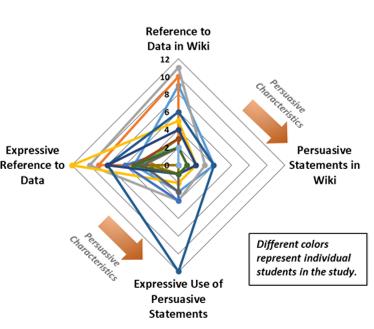
\includegraphics[width=1\linewidth]{Fig 1.png}
    \caption{Cohort two class vector of student usage of scientific argumentation}
\end{figure}

Another component of scientific argumentation is represented by the ability to identify, utilize, and leverage data and evidence within the constraints of pursuing a warrant or hypothesis. Researchers have demonstrated that students who reference specific data and evidence are more likely to build upon them and include persuasive statements (Berland \& Reiser, 2009). Figure 1 demonstrates that all students who gave presentations indeed referenced data and appeared to have understood the value in using evidence to support their claims, as they included at least two references to data throughout their wiki writing and presentations. However, students did not consistently build upon the data references to construct persuasive statements. Overall, the majority of these students were well-versed in referencing data in their wikis and presentations, though some without explicit connection to arguments made in their wikis. 

Though the majority of the students referenced data within their wiki writing and throughout their expressive presentations, it is important to note that students were not taught explicitly, nor coached, on how to use persuasive statements in their presentations or their writing. Rather, students were generally instructed to “persuade your instructor/peers of your position on climate change.” There was no explicit instruction offered to students regarding the differences in genre and writing components of persuasion versus explanations. Our analysis revealed that teaching assignments, lectures, and evaluation rubrics and assessments emphasized reference to raw data often above argumentation. We noted that student data (both in the wiki and during the presentations) was often wielded without the explicit reasoning nor backing behind it that would directly connect evidence to warrants and hypotheses. In this way, persuasive statements sometimes subverted the introduction and support of argumentation in general. 

We interviewed students to ensure that we correctly understood their perspectives of their experiences throughout the assignment. We did so through restatement of our findings to these students in order to allow for edits to any perspectives that we may have misinterpreted. Our results revealed that students attempted to be successful in the classroom tasks by employing argumentation strategies that they had either been taught or had been exposed to in prior educational experiences (but most of the students reported that they had not previously been exposed to such strategies). As a result of differences in their high school preparation, students appropriated argumentation to varying degrees of success. The initial coding process prompted us to explore more of the students’ prior experiences learning science and modes through which they had previously been engaged in science classroom discourse. Our compilation of students’ contributions from presentation and writing samples illuminated important differences in the ways students had learned. The process provided perspective regarding where students may be lacking in their attempts to move from sense-making, to articulation, and then to persuasion.

\subsubsection*{Students who used persuasive statements.}

The follow-up interviews with students in the second cohort revealed that some students had experienced deeper and richer forms of classroom discourse in their academic preparation, while many others were relegated to traditional classroom experiences that is documented throughout the literature (Lemke, 1990; Sinclair \& Coulthard, 1975). This subset of students approached the classroom assigned tasks and classroom interactions through an orientation of persuasion and a use of available evidence for the construction of scientific arguments. Using persuasion and evidence-based argument, they approached the mining of evidence, compiling of findings, and presented their projects as a means to persuade an implied audience. Given the same ACS Toolkit resource and the same task of constructing an argument regarding climate science literacy, these students created significantly different writing products and generally reported it as a much more valuable experience than their contrasting group. 

Like most students in the study, “Nancy” performed largely with ‘explainer’ characteristics (but as explained, there is an argumentation range in which students can be placed), but comparatively she used relatively more persuasive statements than her classmates. She used persuasive statements throughout the wikis and presentation. She also widely used referenced evidence and, through her expressive articulation of data sources, articulated responses and rebuttals to her real or imagined critics. Nancy demonstrated a quality use of argumentation in her individual and collaborative contributions to the classroom. Her vector of argumentation responses is shown in Figure 2. Unlike most of her peers, Nancy was exposed to argumentation strategies in her prior education experiences.

\begin{figure}[h]
    \centering
    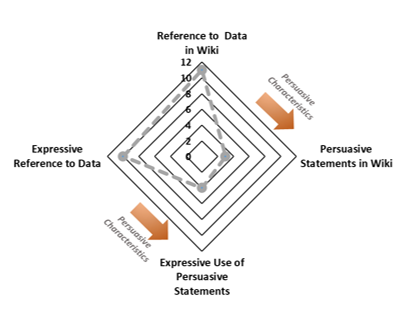
\includegraphics[width=1\linewidth]{Fig 2.png}
    \caption{Nancy’s scientific argumentation vector}
\end{figure}

In describing her learning process, Nancy expressed enjoyment in completing the task and satisfaction with her work. Nancy welcomed the challenge to “persuade your peers” and she valued the opportunity to present to her peers what she had learned and created in her wiki. It was also her feeling that many of her peers’ efforts were minimal and not “investing themselves” or “living up to the standard” that the instructor had set. When asked if she could postulate why she had little trouble composing her argument for climate change but her peers had less success, she surmised, 
\begin{quote}
    Nancy:  “Well…I think maybe why they are not using persuasive statements, because they were trying their best on answering the questions. Not focus on proving who they are presenting to. They are focusing on answering the question, find the answer, put it down, answer the questions, that’s it…”
\end{quote}

“Robert,” who performed admirably as a ‘persuader’, was a primary-ASL signer, who demonstrated the most prolific use of persuasive statements during the presentation. He used phrases like “…shows that climate change is happening,” and “This picture shows how humans impact the earth…” Robert used a relatively high number of appropriate persuasive statements and only an average number of references to data in the wiki and presentation. He stated in interviews that he knew how to use persuasive statements because of his background and practice with his former teacher from high school. Robert’s argumentation vector (Figure 3) demonstrates a strong contingent of argumentation strategies measured, and when asked, he described how he approached his task. He said that he had actually practiced by “…finding other people [in class and in public] and practiced persuading them of how we cause climate change.” 

\begin{figure}[h]
    \centering
    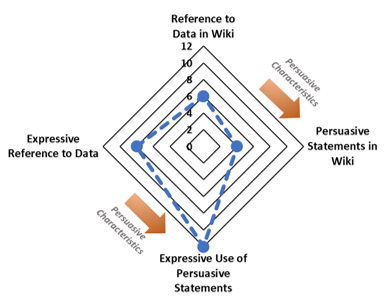
\includegraphics[width=1\linewidth]{Fig 3.png}
    \caption{Robert’s scientific argumentation vector}
\end{figure}

\subsubsection*{Students who predominantly explained/stated facts.}

In contrast to ‘persuaders’, some students (also in the second cohort) approached their climate science assignments as tasks to recall and to restate previously documented information and knowledge. They became ‘explainers’ to their peers as they collected and reconstituted existing knowledge by fact-checking. In fact, one student described their motivation to “compete and to develop the best wiki to achieve the ‘A’ grade” as opposed to being motivated to learn the topic. When Deaf and hard-of-hearing students were required to write and post collective reasoning in a wiki format, these ‘explainers’ summarized the visuals by explaining the facts within and directed the readers’ attention to other factual resources elsewhere. The data collected from ‘explainers’ often revealed no use of persuasive statements, they instead collectively approached the task to explain climate change information they had harvested from assigned web resources within the ACS Toolkit. 

An example of a student who responded as an ‘explainer’ is Rose. As multiple students referenced in interviews, like Rose, they were not taught how to use persuasive statements in the past. She was very interested in doing the climate change project and claimed that she “learned a lot.” Throughout her interview, she clarified that she focused on sharing data and images that “people cared about.” She believed she had a good wiki to persuade her classroom peers:

\begin{quote}
    Rose: “I thought that my project was good…that like it was good to learn from…” \\
Invw: What about your project did you think was good? What convinced yourself that you had a good project? \\
Rose: “I remember I had a lot of facts, like a lot of resources, like online...I remember it was online…” \\
Invw: the ACS website? \\
Rose: “yes, that”
\end{quote}

Rose also explained her approach in addition to finding images “people cared about,” was to use strategies she used in lab reports:

\begin{quote}
Rose: “and…also did, like we were using in lab report, I did ‘figure one’, ‘based on figure one, or ‘table one,’ or something like that…I’m used to that from lab reports.” \\
Invw: You learned that in college, correct, not in high school, right? \\
Rose: “right, in high school was more like ‘table one,’ but we didn’t mention anything about it, we just showed what it was and that, that was it…um…high school was pretty much, you didn’t talk about the data itself, you just show it…”
\end{quote}

As demonstrated in these quotes from Rose, she used what she had learned in school, applied what she believed were good ways to persuade by using references to data and images that would “move” her peers (an attribute that might typically be ascribe to a ‘persuader’). However, like other students mentioned, since she had not been explicitly taught strategies like using persuasive statements, she predominantly groups as an ‘explainer’. As can be seen in her argumentation vector (Figure 4), Rose did not use any persuasive statements in her wiki writing, nor did she during her presentation.

\begin{figure}[h]
    \centering
    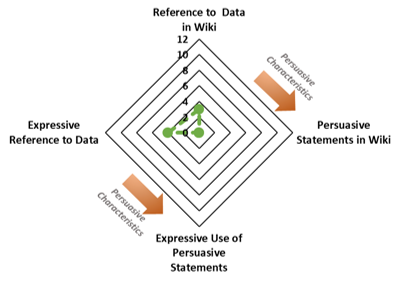
\includegraphics[width=1\linewidth]{Fig 4.png}
    \caption{Rose’s scientific argumentation vector}
\end{figure}
\newpage
Our case study suggests that given the expectation for students to develop the ability to create scientific arguments and effectively communicate them, Deaf and hard-of-hearing students, as ‘explainers’ and ‘persuaders’, approach such goals differently. We found that Deaf and hard-of-hearing students may often approach persuasion tasks from the perspective of an ‘explainer’. Our interviews with students suggested that these students had not been exposed to making persuasive statements in their prior education. Without intervening, these students may not develop the argumentation skills for use in the field (e.g. persuading fellow scientist about the implications from an evidence-based study). In contrast, those who are ‘persuaders’ led to the development of argumentation skills that might be akin to professional scientists in the field. These are also the skills needed for an environmental science-literate citizenry.

\section*{CONCLUSION}

As we use a sociocultural framework to come to understand the characteristics of certain groups of learners, whether they be ‘explainers’, ‘persuaders’, or whatever category emerges in the examination of our students and teaching, to guide our instructional practices as we make sense of how our students interpret what we \textit{think} we are teaching them would prove valuable. Most students were excited and motivated by the opportunity to create and to engage differently with content than they did in prior classroom experiences. However, students demonstrated different levels of mastery related to argumentation skills. Some students were very compelling and persuasive with their peers, while some never made a single persuasive statement—even though the second cohort of students were instructed to “persuade your instructor/peers.” Several students compiled, and deeply analyzed, collections of data that bolstered the argument that they defended, while other students concentrated on creating pleasant, visually appealing wikis with vast amounts of factual information. Regardless of what we intend, we as teachers can never fully determine what students will do with our assignments. We must explore and reflect to discover more about our learners. 

We noticed as we reviewed the classroom videos that the students were never directly coached on strategies to change or edit their wikis in order to be more persuasive. We did not see in the teaching episodes what could be explained as a deconstruction in front of students of what a persuasive statement does or does not look like. If students had experiences in their past that made such discourse explicit, they would certainly be at an advantage in this task. This justifies the need for teachers to give instruction related to scientific argumentation, which we definitely plan to do in the future, but was not the goal of our study. 

Gee (1989) makes a clear separation about how discourses, like argumentation, are \textit{acquired} and how this process is different from how we typically \textit{learn} in school. Gee claims that we are better at practicing what we have acquired, but we know more about what we have learned. In this way, Gee is suggesting that learning and acquisition are different cognitive processes. Through this lens, we should expect that my students who have memorized, recalled, and \textit{learned} information would remember and know more. They might be predominantly ‘explainers’ and they might have successfully done this throughout their entire student careers. We would also expect that ‘persuaders’ would recognize and dive into opportunities to persuade others if they have had such opportunities before and/or been engaged in debate or scientific inquiry, and therefore, likely demonstrate that they have \textit{acquired} this kind of discourse. 

When it comes to the acquisition of science discourse in the education of students with disabilities, we face an issue where we need to provide CRT. Yet, the challenge and premise of each of the last two science education reforms (i.e. Common Core State Standards and NGSS) has been inclusivity, equity, and “Science for All Americans”. Part of my student population doesn’t seem to be getting access and exposure to this kind of learning. It is important to consider the lack of access to argumentation practices by the primary-ASL learners. Our study helps to establish the need for providing access to scientific argumentation practices for Deaf and hard-of-hearing learners. If these are the standards for the NGSS, then Deaf and hard-of-hearing students need more exposure to argumentation in science curricula– though what might be considered effective techniques in the traditional classroom, may not be as effective to the Deaf and hard-of-hearing community (and \textit{vice versa}). Especially in emergent technical and socially important fields, like sustainability environmental science, change is required in the form of establishing culturally-responsive educational initiatives. 

\section*{LIMITATIONS}

As might be expected with this low-incidence population, this case study involved a relatively small sample. Therefore, student demographic information has been withheld for privacy of the participants. Incidentally, the student groups had diversity in language preferences and educational backgrounds— so, the group wasn’t entirely uniform in those respects. Essentially, the NTID students in our study are all Deaf and hard-of-hearing and arrived to campus from  several states within the U.S. These students have a mixed background of communication preferences, including oral/hard-of-hearing (no sign language knowledge), oral/Deaf and hard-of-hearing (no sign language knowledge), Deaf and hard-of-hearing (use of ASL), and Hard-of-hear-ing (use of ASL). As a result, they represent a conglomeration of primary-ASL language users and primary-English language users. These students also have a variety of access service preferences (ASL interpreting, captioning, etc.). This array of language needs/preferences makes the instructional process challenging in that not only is the instructor required to address the needs of a potentially ELL classroom, but also the fact that ASL has no written component to it, making English the default (but often not favored) written form of communication. 

While there were two cohorts studied, the earlier cohort worked in teams, rather than individually, and they were not specifically instructed to persuade—so these differences make comparisons between the two cohorts difficult. Thus, the discussion on Cohort One focused on their interviews and how the two groups of ‘persuaders’ and ‘explainers’ were found throughout the coding process.  The discussion related to Cohort Two focused on counts (vectors) of their written and explanatory presentations, in addition to interviews with students from this group.

Throughout the project, another limitation is that students were provided the ACS toolkit in the English language only—not in ASL. Thus, the language proficiency of the students as they developed their written wiki and explanatory presentations might have impacted their understanding, as well as their relaying of the information and data from the ACS toolkit. 

\subsection*{ACKNOWLEDGMENTS:} The authors would like to thank Camille Ouellette and Thomastine Sarchet for their contributions throughout the study. Additionally, we thank the American Chemical Society for the availability of the Climate Science Website for the study.

\end{large}
\clearpage
\section*{References}\par 

\begin{hangparas}{0.25in}{1}

Abes, E. S., \& Wallace, M. M. (2018). “People See Me, But They Don’t See Me”: An Intersectional Study of College Students with Physical Disabilities. \textit{Journal of College Student Development; Baltimore, 59}(5), 545–562. 

Abrokwa, A. (2018). “When They Enter, We All Enter”: Opening the Door to Intersectional Discrimination Claims Based on Race and Disability. \textit{Michigan Journal of Race \& Law; AnnArbor,24}(1),15–74.

ACS Climate Science Toolkit—American Chemical Society. (2008). Retrieved July 28, 2015, from \url{http://www.acs.org/content/acs/en/climatescience.html}

Barcroft, J., \& Wong, W. (2013). Input, input processing and focus on form. In M. Herschensohn \& M. Young-Scholten (Eds.), \textit{The Cambridge Handbook of Second Language Acquisition} (1sted.).

Bell, P., \& Linn, M. C. (2000). Scientific Arguments as Learning Artifacts: Designing for Learning from the Web with KIE (Knowledge Integration Environment). \textit{International Journal of Science Education, 22}(8), 797–817.

Berland, L. K., \& Reiser, B. J. (2009). Making sense of argumentation and explanation. \textit{Science Education, 93}(1), 26–55.

Buckley, J. B. (2019). A Grounded Theory of Education for Sustainability in the Postsecondary Classroom.\textit{Revie-wofHigherEducation,42}(3),965–989. 

Cannon, J. E., \& Guardino, C. (2012). Literacy Strategies for Deaf/Hard-of-Hearing English Language Learners: Where Do We Begin? \textit{Deafness \& Education International, 14}(2), 78–99. 

Cavagnetto, A. R., \& Kurtz, K. J. (2016). Promoting Students’ Attention to Argumentative Reasoning Patterns. \textit{Science Education, 100}(4), 625–644.

Connolly, P. H., \& Vilardi, T. (Eds.). (1989). \textit{Writing to learn mathematics and science.} New York: Teachers College Press, Teachers College, Columbia University.

Duschl, R. A., \& Osborne, J. (2002). Supporting and promoting argumentation discourse in science education. \textit{Studies in Science Education; Leeds, 38}, 39. 

Emmorey, K. (2002). \textit{Language, Cognition, and the Brain: Insights from Sign Language Research}. Mahwah, N.J: Lawrence Erlbaum Associates.

Erickson, F. (2012). Qualitative Research Methods for Science Education. In B. J. Fraser, K. Tobin, \& C. J. McRobbie (Eds.), \textit{Second International Handbook of Science Education} (pp. 1451–1469). 

Gee. (1989). What is Literacy. \textit{Journal of Education, 171}(1), 18–25.

Grooms, J., Sampson, V., \& Enderle, P. J. (2018). How Concept Familiarity and Experience with Scientific Argumentation are Related to the Way Groups Participate in an Episode of Argumentation. \textit{Journal of Research in Science Teaching, 55}(9), 1264–1286.

Kanwar, T., \& Asad, H. (2019). The need for environmental sustainability in our curriculum. \textit{Medical Teacher}, 1–1. 

Kerschbaum, S. L., \& Price, M. (2017). Centering Disability in Qualitative Interviewing. \textit{Research in the Teaching of English; Urbana, 52}(1), 98–107. 

Knoors, H. (2013). \textit{Teaching deaf learners: Psychological and developmental foundations}. Oxford: Oxford University Press.

Lemke, J. L. (1990). \textit{Talking Science: Language, Learning, and Values}. Westport, Conn: Ablex Publishing Corporation.

Linn, M. C. (1995). AERA SIG: Education, Science and Technology: Designing Computer Learning Environments for Engineering and Computer Science: The Scaffolded Knowledge Integration Framework. \textit{Journal of Science Education and Technology, 4}(2), 103–126. 

Lozano, R., Barreiro-Gen, M., Lozano, F. J., \& Sammalisto, K. (2019). Teaching Sustainability in European Higher Education Institutions: Assessing the Connections between Competences and Pedagogical Approaches. \textit{Sustainability, 11}(6), 1602. 

Marschark, M., Tang, G., \& Knoors, H. (Eds.). (2014). \textit{Bilingualism and Bilingual Deaf Education}. New York, NY: Oxford University Press.

Mayer, C., \& Akamatsu, C. T. (1999). Bilingual-bicultural Models of Literacy Education for Deaf Students: Considering the Claims. \textit{Journal of Deaf Studies and Deaf Education, 4}, 1–8.

McNeill, Katherine L., \& Krajcik, J. (2009). Synergy Between Teacher Practices and Curricular Scaffolds to Support Students in Using Domain-Specific and Domain-General Knowledge in Writing Arguments to Explain Phenomena. \textit{Journal of the Learning Sciences, 18}(3), 416–460. 

McNeill, K.L, Gonzalez, H. M., Katsh-Singer, R., \& Loper, S. (n.d.). Moving Beyond Pseudoargumentation: Teachers’ Enactments of an Educative Science Curriculum Focused on Argumentation. \textit{Science Education, 101}(3), 426–457.

McNeill, K.L, Lizotte, D., Krajcik, J., \& Marx, R. (2006). Supporting students’ construction of scientific explanations by fading scaffolds in instructional materials. \textit{The Journal of the Learning Sciences, 15}(2), 153–191.

Mishler, E. G. (1986). \textit{Research Interviewing: Context and Narrative}. Cambridge, MA: Harvard University Press.

Munro, L., Knox, M., \& Lowe, R. (2008). Exploring the Potential of Constructionist Therapy: Deaf Clients, Hearing Therapists and a Reflecting Team. \textit{The Journal of Deaf Studies and Deaf Education, 13}(3), 307–323. 

National Governors Association Center for Best Practices, \& Council of Chief State School Officers. (2010). \textit{Common Core State Standards}. Washington D.C.: National Governors Association Center for Best Practices, council of Chief State School Officers.

NGSS Lead States. (2013). \textit{Next Generation Science Standards: For States, By States (2013)}. National Academies Press.

NTID. (2018). National Technical Institute for the Deaf Annual Report. Retrieved from \url{https://www.ntid.rit.edu/sites/default/files/annual/_report/_2018.pdf}

Nuwagaba, E. L., \& Rule, P. N. (2016). An adult learning perspective on disability and microfinance: The case of Katureebe. \textit{African Journal of Disability; Pretoria, 5}(1), 1–10. 

Oliver, M. (1986). Social Policy and Disability: Some Theoretical Issues. \textit{Disability \& Society, 1}(1), 5–17.

Pagano, T. (2017). Making Education and Careers in Chemistry Accessible and Successful for Deaf and Hard-of-Hearing Students. In Nelson \& Cheng (Series Ed.), \textit{Diversity in the Scientific Community} (pp. 125–132). Washington, D.C.: American Chemical Society.

Pagano, T., Ross, A. D., \& O’Neill, G. J. (2012). A Program Like Any Other-Like None Other: The Laboratory Science Technology Program for Deaf and Hard-of-Hearing Students. \textit{Journal of Science Education for Students with Disabilities, 15}(1), 11–25.

Plaza-Pust, C. (2014). Language Development and Language Interaction in Sign Bilingual Language Acquisition. In \textit{Bilingualism and Bilingual Deaf Education} (pp. 23–53). Oxford University Press.

Quinn, H., Lee, O., \& Valdes, G. (2012). Language Demands and Opportunities in Relation to Next Generation Science Standards for English Language Learners: What Teachers Need to Know.\textit{ Language, Literacy and Learning in the Content Areas,} 1–12. Stanford, CA: Stanford University.

RIT/NTID ASL CORE. (2019). Retrieved from \url{https://aslcore.org/sustainability/}

Ross, A. D., Yerrick, R., \& Pagano, T. (2019). Assessment of Climate Science Knowledge and Perceptions of Deaf and Hard-of-Hearing Students. \textit{Journal of Science Education for Students with Disabilities}, in press.

Ross, A., Yerrick, R., \& Pagano, T. (2019). Examining the use of Argumentation Strategies in Deaf/Hard-of-Hearing Learning Contexts to Teach Climate Science. In \textit{Communication in Chemistry}. Accepted.

Sampson, V., \& Walker, J. P. (2012). Argument-Driven Inquiry as a Way to Help Undergraduate Students Write to Learn by Learning to Write in Chemistry. \textit{International Journal of Science Education, 34}(10), 1443–1485. 

Sinclair, J., \& Coulthard, R. M. (1975). \textit{Toward an Analysis of Discourse}. Oxford: Oxford University Press.

Singleton, J., Morgan, D., DeGello, E., Wiles, J., \& Rivers, R. (2004). \textit{Vocabulary use by low, moderate, and high ASL-proficient writers compared to hearing ESL and monolingual speakers. 9}, 86–103.

Snyder, T. D., de Brey, C., \& Dillow, S. A. (2016). \textit{Digest of Education Statistics 2016 (NCES 2017-094)}. Washington, DC: National Center for Education Statistics, Institute of Education Sciences, U.S. Department of Education.

Spradley, J. (1980). \textit{Participant Observation}. United States -- California: Wadsworth Cengage-Learning.

SRI International. (2006a). \textit{NLST2 Wave 2 Student School Program Survey Student Achievement-Reading Ability}. Retrieved from \url{http://www.nlts2.org/data\_tables/tables/9/npr2B2bfrm.html}

SRI International. (2006b). \textit{NLST2 Wave 2 Student School Program Survey Student Achievement-Math Ability}. Retrieved from \url{https://nlts2.sri.com/data\_tables/tables/9/npr2B3bfrm.html}

Stokoe, W. C. (1978). \textit{Sign Language structure: The first linguistic analysis of American sign language}. Silver Spring, MD: Linstok Press.

Tejedor, G., Segalas, J., Barron, A., Fernandez-Morilla, M., Teresa Fuertes, M., Ruiz-Morales, J., Hernandez, A. (2019). Didactic Strategies to Promote Competencies in Sustainability. \textit{Sustainability, 11}(7), 2086. 

Tolbert, S., Stoddart, T., Lyon, E. G., \& Solis, J. (2014). The Next Generation Science Standards, Common Core State Standards, and English Learners: Using the SST-ELLA Framework to Prepare Secondary Science Teachers.\textit{ Issues in Teacher Education; San Bernadino, 23}(1), 65–90. 

U. S. Census Bureau. (2013) \textit{Disability Characteristics 2013-2017 American Community Survey 5-Year Estimates}. Retrieved from \url{https://factfinder.census.gov/faces/tableservices/jsf/pages/productview.xhtml?pid=ACS\_17\_5YR\_S1810\&prodType=table}

Vygotskiĭ, L. S. (1987). \textit{The collected works of L.S. Vygotsky}. New York: Plenum Press.
\end{hangparas}

\clearpage
\onecolumn

\setcounter{table}{0}
\renewcommand{\thetable}{A\arabic{table}}

\newcolumntype{M}[1]{>{\centering\arraybackslash}m{#1}}
\begin{table*}[!htbp]
\caption{Author's Coding using Spradley (1980).}
\begin{tabular}{|c|c|c|c|c|}
\hline
\# & Terms & Form & Cover Term/Phrase & Evidence \\ \hline
1 & Questioning & Is used for & Inquiry & ``I don’t know which is the worse, is pollution that is the worse?  Is the air the worse? Is the animals going the worse thing?  Where our priorities, which one is really changing the most versus which is not that important.'' \\ \hline
\multirow{3}{*}{2} & Use of Evidence & \multirow{3}{*}{Is a part of} & \multirow{3}{*}{Argumentation} & ``I think the earth itself has its own climate system. Like its’ own…because before us humans were here, we had the earthquakes, the plates were separating, everything, like we can’t control the earthquakes, we can’t do that, that’s not from us, like we can’t control that.'' \\ \cline{2-2}\cline{5-5}
& Fact Checking & & & “… go online check…” \\ \cline{2-2}\cline{5-5}
& Determination of which evidence is relevant & & &  “…figuring out what’s important.” \\ \hline
8 & Attention to Type of Audience & Is a reason for doing & Changes in expressive scientific discourse & “…I have to figure out what kind of audience, if it’s like a scientific audience, that means to change the words, make it more smart, more understanding, more clear, facts, not vague.” \\ \hline
\multirow{2}{*}{3} & Working with other students & \multirow{2}{*}{Is a way to do} & \multirow{2}{*}{Peer writing} & “To help with my writing…with working with other students, because we all saw the same presentation at the same time, so if we were on different, different computers,” \\ \cline{2-2}\cline{5-5}
& Checking grammar & & & “…definitely checking grammar…” \\ \hline
5 & ACS wiki format & Is used for & Organization of Knowledge & ``Honestly, I liked this Toolkit, it wasn’t easy, no, but it was easier in a way of more organizing information than a lot of other teachers do.'' \\ \hline
\multirow{2}{*}{6} & Divided ACS website information up to each team member & \multirow{2}{*}{Is a way to do} & \multirow{2}{*}{Groupwork} & “We had to figure out our topics, and I think, what happened, we figured out our topics, and hopefully figured out our themes.” \\ \cline{2-2} \cline{5-5}
& Working together & & & “…and then we put it together, and then we checked our presentation, make sure it flows,” \\ \hline
\multirow{3}{*}{7} & \multirow{3}{*}{Evidence is the same as terms} & Is a kind of & Goal & “…for how to explain how climate change is happening to our earth, that concept…” \\ \cline{3-5}
& & Is a kind of & Evidence for learning &  “Understanding more clearly…” \\ \cline{3-5}
& & Is a part of & Positioning Theory & “…because I’ve noticed from society, people look down on bad grammar.” \\ \hline
8 & Audience determination & Is a reason for doing & Changes in expressive scientific discourse & “…, I have to figure out what kind of audience, if it’s like a scientific audience, that means to change the words, make it more smart, more understanding, more clear, facts, not vague.” \\ \hline
9 & Class Presentations on content & Is a step in & Understanding that content & “But, it was nice because my presentation, their presentations were all connected, because we could see the connections in CLIMATE CHANGE ideas.” \\ \hline
10 & Pictures, links to other websites on the ACS wiki & Is a way to do & Multi-model learning & “It expanded a lot more, with pictures, it was nice.“ \\ \hline
11 & Speech & Is used for & Learning grammar & ``And plus my speech is good, so I learned my grammar that way, so sometimes I would read their words and it wouldn’t make sense to me, because their grammar is not appropriate.'' \\ \hline
\end{tabular}
\end{table*}
\end{document}